\documentclass[tikz,border=12pt]{standalone}

\usepackage{tikz}
\usetikzlibrary{
  shapes.geometric, shapes.misc,
  arrows.meta, arrows,
  positioning, fit, calc,
  backgrounds, shadows
}
\usepackage{amsmath,amssymb}
\usepackage{xcolor}
\usepackage[T1]{fontenc}

%% ── Color Palette ────────────────────────────────────────────
\definecolor{navyblue}{RGB}{20,60,120}
\definecolor{midblue}{RGB}{60,120,190}
\definecolor{coralred}{RGB}{210,80,70}
\definecolor{mintgreen}{RGB}{60,160,110}
\definecolor{amber}{RGB}{200,140,30}
\definecolor{lavender}{RGB}{120,90,170}
\definecolor{deepteal}{RGB}{20,100,100}
\definecolor{boxblue}{RGB}{210,225,245}
\definecolor{boxred}{RGB}{245,215,215}
\definecolor{boxorange}{RGB}{255,232,205}
\definecolor{boxgray}{RGB}{228,228,228}
\definecolor{boxgreen}{RGB}{200,235,210}
\definecolor{boxpurple}{RGB}{228,215,242}
\definecolor{cDark}{RGB}{40,60,100}
\definecolor{fusioncolor}{RGB}{200,80,20}
\definecolor{rlblue}{RGB}{30,90,160}
\definecolor{rlgreen}{RGB}{20,140,60}
\definecolor{memorycol}{RGB}{200,180,240}
\definecolor{qnetcol}{RGB}{170,210,250}
\definecolor{actioncol}{RGB}{245,220,170}
\definecolor{nlpcol}{RGB}{200,240,200}
\definecolor{sectionA}{RGB}{235,245,255}
\definecolor{sectionB}{RGB}{255,245,235}
\definecolor{sectionC}{RGB}{235,255,240}
\definecolor{sectionD}{RGB}{255,235,245}
\definecolor{sectionE}{RGB}{245,240,255}
\definecolor{sectionRAG}{RGB}{255,250,230}
\definecolor{sectionRL}{RGB}{240,255,245}

%% ── Node Styles ─────────────────────────────────────────────
\tikzset{
  basebox/.style={rectangle,rounded corners=5pt,draw=black!50,align=center,font=\small},
  inputnode/.style={basebox,fill=cDark,text=white,minimum width=3.0cm,minimum height=1.1cm,font=\small\bfseries},
  encnode/.style={basebox,fill=boxblue,draw=navyblue!70,minimum width=3.0cm,minimum height=1.0cm,thick},
  projnode/.style={basebox,fill=boxorange,draw=amber!80,minimum width=3.0cm,minimum height=1.0cm,thick},
  retnode/.style={basebox,fill=boxgreen,draw=mintgreen!80,minimum width=3.0cm,minimum height=1.0cm,thick},
  gennode/.style={basebox,fill=boxred,draw=coralred!80,minimum width=3.0cm,minimum height=1.0cm,thick},
  outnode/.style={basebox,fill=boxpurple,draw=lavender!80,minimum width=3.0cm,minimum height=1.0cm},
  fusnode/.style={basebox,fill=fusioncolor!15,draw=fusioncolor!70,minimum width=3.2cm,minimum height=1.0cm,thick},
  decnode/.style={diamond,draw=amber!90,fill=yellow!25,aspect=2.8,align=center,font=\small\bfseries,minimum width=3.0cm,minimum height=1.2cm},
  datanode/.style={basebox,fill=boxgray,draw=black!40,minimum width=2.8cm,minimum height=0.9cm,font=\small},
  lossnode/.style={basebox,fill=boxorange,draw=amber!80,minimum width=3.0cm,minimum height=1.0cm},
  qnetnode/.style={basebox,fill=qnetcol,draw=rlblue,minimum width=3.0cm,minimum height=1.2cm,thick},
  memnode/.style={basebox,fill=memorycol,draw=lavender,minimum width=3.0cm,minimum height=1.0cm},
  robotnode/.style={basebox,fill=actioncol,draw=amber,minimum width=3.0cm,minimum height=1.0cm,thick},
  nlpnode/.style={basebox,fill=nlpcol,draw=mintgreen,minimum width=3.0cm,minimum height=1.0cm},
  seclabel/.style={font=\normalsize\bfseries},
  phaselabel/.style={font=\small\bfseries},
  arr/.style={->,>=Stealth,thick,color=black!70},
  thickarr/.style={->,>=Stealth,very thick,color=cDark},
  redarr/.style={->,>=Stealth,thick,color=coralred!80},
  greenarr/.style={->,>=Stealth,thick,color=mintgreen!80},
  bluearr/.style={->,>=Stealth,thick,color=rlblue},
  dasharr/.style={->,>=Stealth,thick,dashed,color=gray!70},
  ambarr/.style={->,>=Stealth,thick,dashed,color=amber!90}
}

\newcommand{\R}{\mathbb{R}}
\newcommand{\Sph}{\mathbb{S}}

\begin{document}
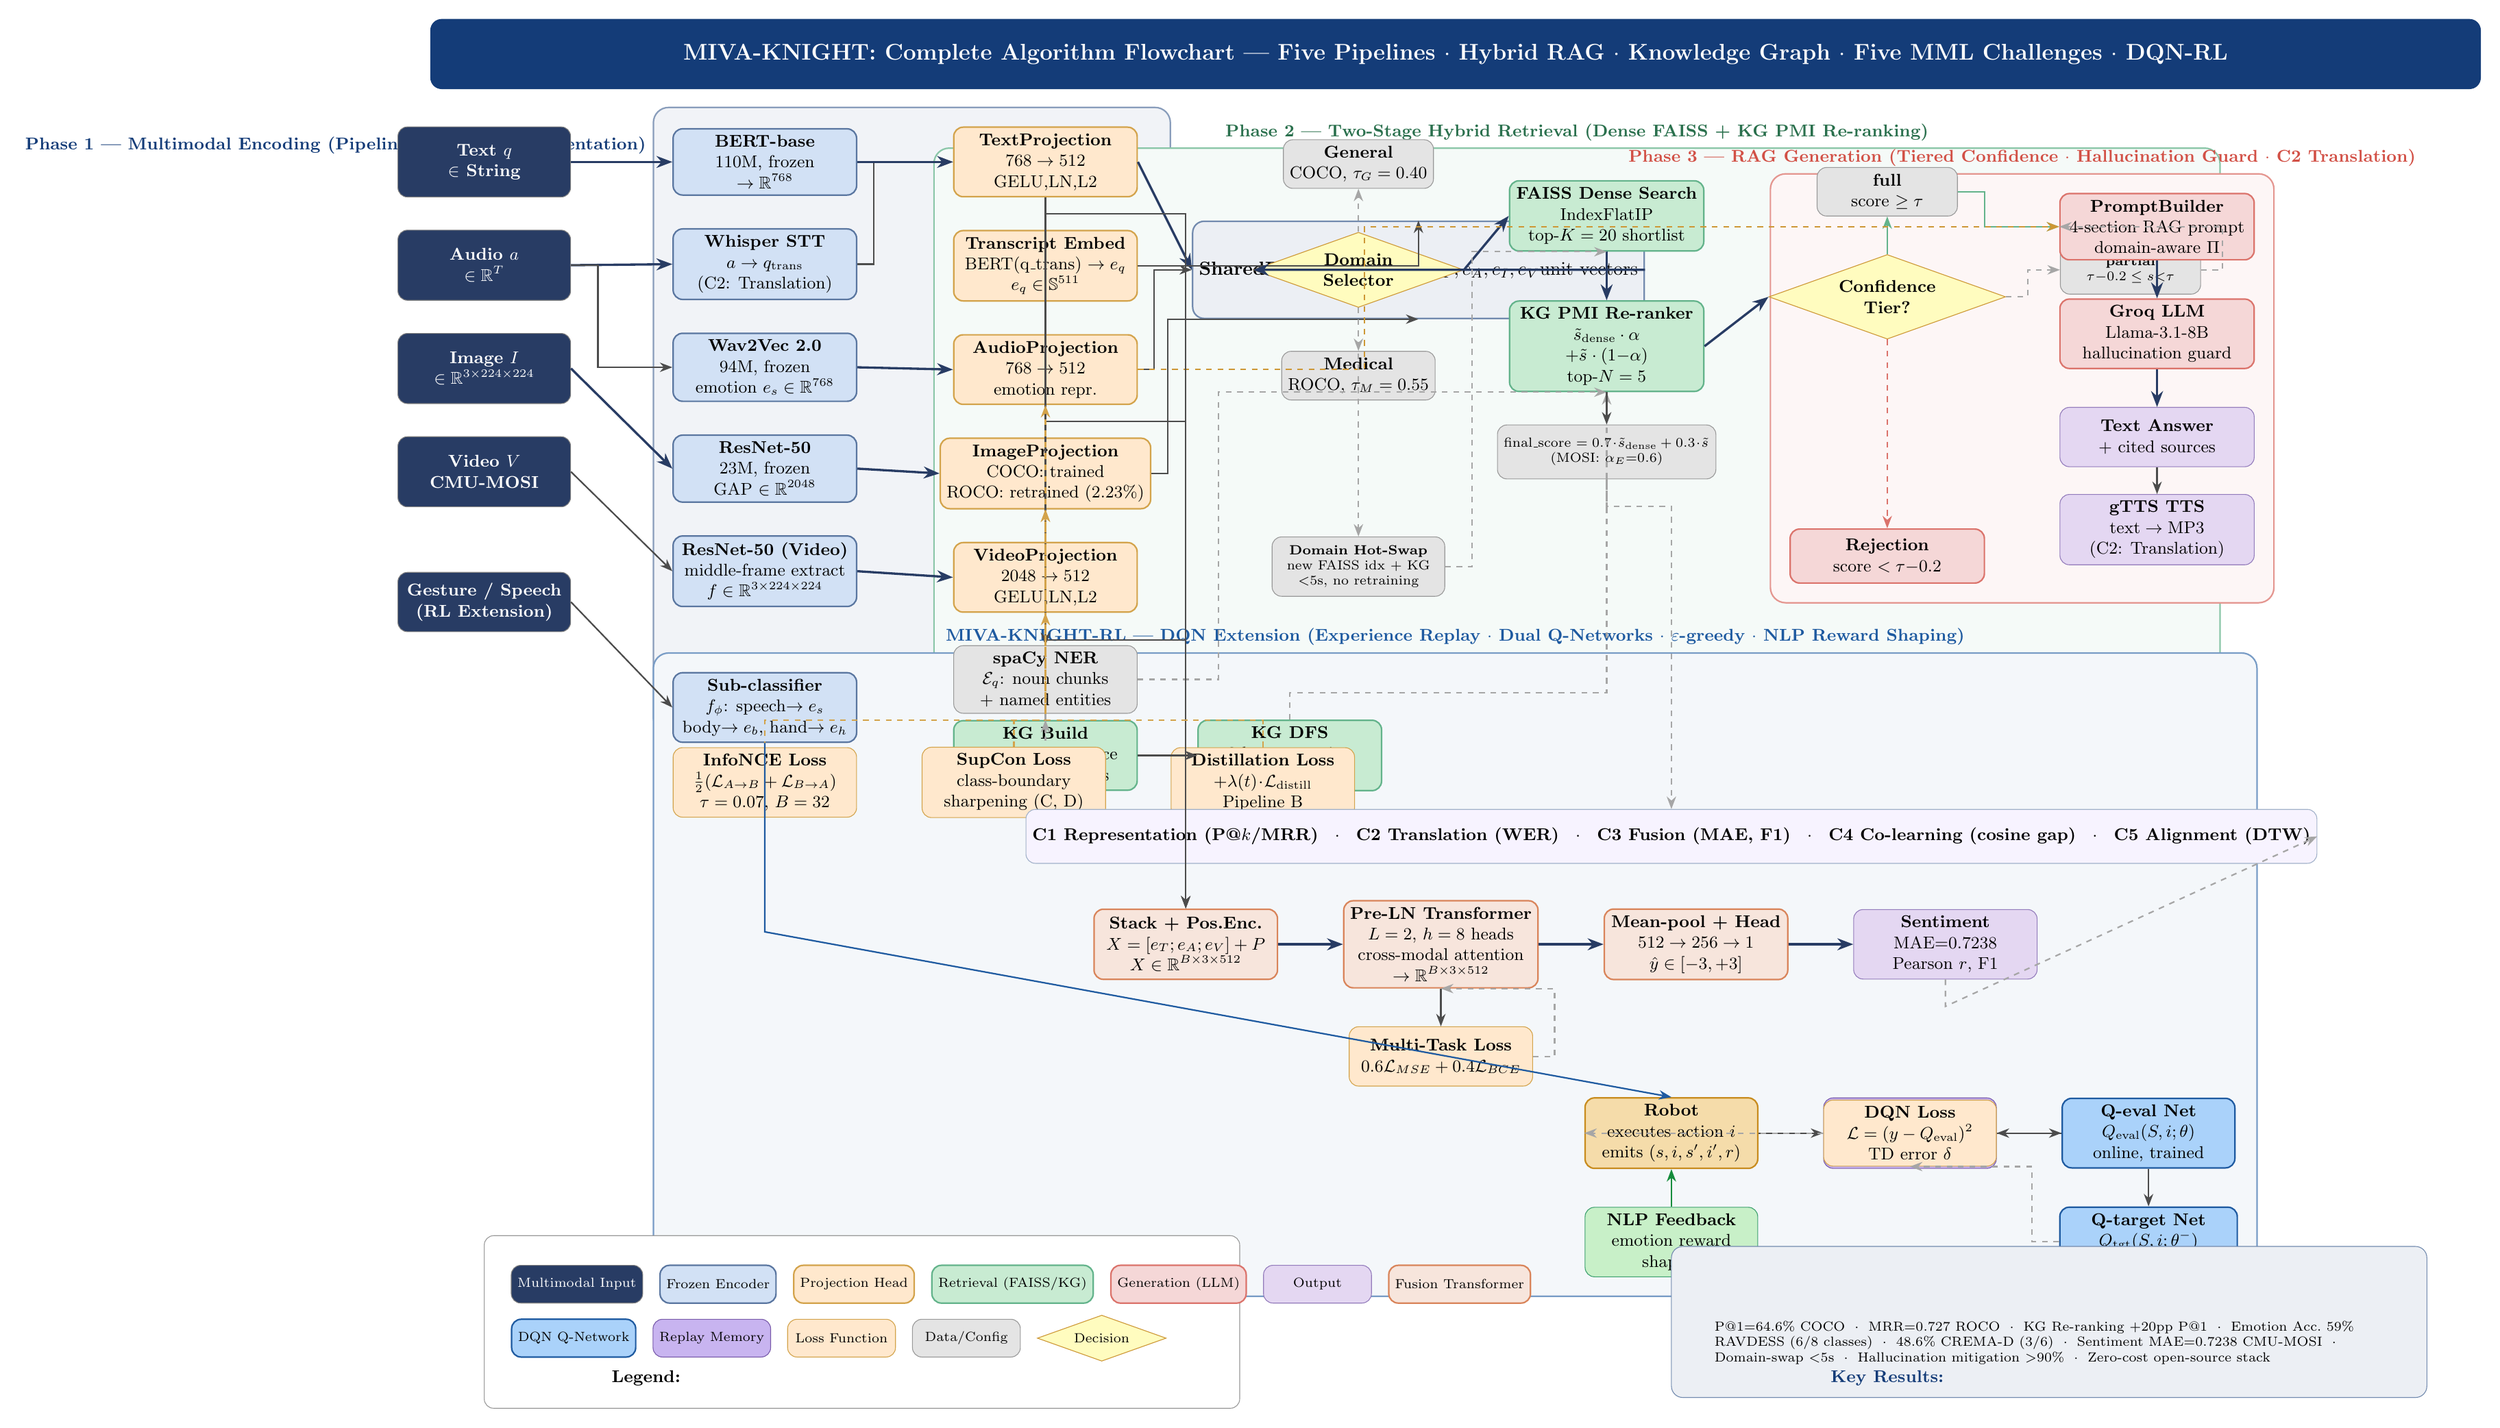
\begin{tikzpicture}[node distance=0.7cm and 1.2cm]

%%=============================================================
%% TITLE BANNER (top)
%%=============================================================
\node[rectangle,fill=navyblue,text=white,font=\large\bfseries,
      minimum width=38cm,minimum height=1.3cm,rounded corners=6pt]
  (title) at (18,2) {MIVA-KNIGHT: Complete Algorithm Flowchart ---
  Five Pipelines $\cdot$ Hybrid RAG $\cdot$ Knowledge Graph $\cdot$ Five MML Challenges $\cdot$ DQN-RL};

%%=============================================================
%% COLUMN 1: MULTIMODAL INPUT BLOCK  (x≈0)
%%=============================================================
\node[inputnode,minimum width=3.2cm,minimum height=1.3cm]
  (textIn) at (0,0) {\textbf{Text} $q$\\$\in$ String};
\node[inputnode,minimum width=3.2cm,minimum height=1.3cm,below=0.6cm of textIn]
  (audioIn) {\textbf{Audio} $a$\\$\in \R^T$};
\node[inputnode,minimum width=3.2cm,minimum height=1.3cm,below=0.6cm of audioIn]
  (imageIn) {\textbf{Image} $I$\\$\in \R^{3\times224\times224}$};
\node[inputnode,minimum width=3.2cm,minimum height=1.3cm,below=0.6cm of imageIn]
  (vidIn) {\textbf{Video} $V$\\CMU-MOSI};
\node[inputnode,minimum width=3.2cm,minimum height=1.1cm,below=1.2cm of vidIn]
  (gestIn) {\textbf{Gesture / Speech}\\(RL Extension)};

%%=============================================================
%% COLUMN 2: FROZEN ENCODER BACKBONES  (x≈5.0)
%%=============================================================
\node[encnode,minimum width=3.4cm,minimum height=1.2cm]
  (bert) at (5.2,0) {\textbf{BERT-base}\\110M, frozen\\$\to\R^{768}$};
\node[encnode,minimum width=3.4cm,minimum height=1.2cm,below=0.6cm of bert]
  (whisper) {\textbf{Whisper STT}\\$a \to q_{\text{trans}}$\\(C2: Translation)};
\node[encnode,minimum width=3.4cm,minimum height=1.2cm,below=0.6cm of whisper]
  (w2v) {\textbf{Wav2Vec 2.0}\\94M, frozen\\emotion $e_s \in\R^{768}$};
\node[encnode,minimum width=3.4cm,minimum height=1.2cm,below=0.6cm of w2v]
  (resnet) {\textbf{ResNet-50}\\23M, frozen\\GAP $\in\R^{2048}$};
\node[encnode,minimum width=3.4cm,minimum height=1.2cm,below=0.6cm of resnet]
  (resnetV) {\textbf{ResNet-50 (Video)}\\middle-frame extract\\$f \in\R^{3\times224\times224}$};
\node[encnode,minimum width=3.4cm,minimum height=1.2cm,below=1.2cm of resnetV]
  (subclf) {\textbf{Sub-classifier}\\$f_\phi$: speech$\to e_s$\\body$\to e_b$, hand$\to e_h$};

%%=============================================================
%% COLUMN 3: PROJECTION HEADS → Shared S^{511}  (x≈10.2)
%%=============================================================
\node[projnode,minimum width=3.4cm,minimum height=1.2cm]
  (tproj) at (10.4, 0) {\textbf{TextProjection}\\$768\to512$\\GELU,LN,L2};
\node[projnode,minimum width=3.4cm,minimum height=1.2cm,below=0.6cm of tproj]
  (transOut) {\textbf{Transcript Embed}\\BERT(q\_trans) $\to e_q$\\ $e_q\in\Sph^{511}$};
\node[projnode,minimum width=3.4cm,minimum height=1.2cm,below=0.6cm of transOut]
  (aproj) {\textbf{AudioProjection}\\$768\to512$\\emotion repr.};
\node[projnode,minimum width=3.4cm,minimum height=1.2cm,below=0.6cm of aproj]
  (iproj) {\textbf{ImageProjection}\\COCO: trained\\ROCO: retrained (2.23\%)};
\node[projnode,minimum width=3.4cm,minimum height=1.2cm,below=0.6cm of iproj]
  (vproj) {\textbf{VideoProjection}\\$2048\to512$\\GELU,LN,L2};

%% NER node
\node[datanode,minimum width=3.4cm,minimum height=1.1cm,below=0.6cm of vproj]
  (ner) {\textbf{spaCy NER}\\$\mathcal{E}_q$: noun chunks\\+ named entities};

%% Shared embedding space label
\node[rectangle,draw=navyblue!60,fill=navyblue!8,rounded corners=6pt,thick,
      minimum width=3.6cm,minimum height=1.8cm,
      right=1.0cm of tproj,yshift=-2.0cm]
  (shared) {\textbf{Shared}\\\textbf{Embedding}\\$\Sph^{511}$\\$e_q,e_T,e_A,e_I,e_V$\\unit vectors};

%%=============================================================
%% DOMAIN ROUTING  (x≈16)
%%=============================================================
\node[decnode,minimum width=3.4cm]
  (dom) at (16.2,-2.0) {\textbf{Domain}\\Selector};
\node[datanode,minimum width=2.6cm,above=0.8cm of dom]
  (gdom) {\textbf{General}\\COCO, $\tau_G=0.40$};
\node[datanode,minimum width=2.6cm,below=0.8cm of dom]
  (mdom) {\textbf{Medical}\\ROCO, $\tau_M=0.55$};

%%=============================================================
%% KG CONSTRUCTION COLUMN  (x≈10, y low)
%%=============================================================
\node[retnode,minimum width=3.4cm,minimum height=1.2cm]
  (kgbuild) at (10.4,-11.0) {\textbf{KG Build}\\PMI co-occurrence\\top-2000 entities};
\node[retnode,minimum width=3.4cm,minimum height=1.2cm,right=1.1cm of kgbuild]
  (kgdfs) {\textbf{KG DFS}\\2-hop expansion\\$\KG_G / \KG_M$};

%%=============================================================
%% COLUMN 4: TWO-STAGE HYBRID RETRIEVAL  (x≈20)
%%=============================================================
\node[retnode,minimum width=3.6cm,minimum height=1.3cm]
  (faiss) at (20.8,-1.0) {\textbf{FAISS Dense Search}\\IndexFlatIP\\top-$K=20$ shortlist};
\node[retnode,minimum width=3.6cm,minimum height=1.3cm,below=0.9cm of faiss]
  (kgrank) {\textbf{KG PMI Re-ranker}\\$\tilde{s}_{\text{dense}}\cdot\alpha$\\$+\tilde{s}_{\KG}\cdot(1{-}\alpha)$\\top-$N=5$};

%% Hybrid score formula node
\node[datanode,minimum width=3.6cm,minimum height=1.0cm,below=0.6cm of kgrank,font=\scriptsize]
  (hybscore) {final\_score $=0.7\!\cdot\!\tilde{s}_{\text{dense}}+0.3\!\cdot\!\tilde{s}_{\KG}$\\(MOSI: $\alpha_E{=}0.6$)};

%%=============================================================
%% COLUMN 5: TIERED CONFIDENCE  (x≈25)
%%=============================================================
\node[decnode,minimum width=3.4cm]
  (conf) at (26.0,-2.5) {\textbf{Confidence}\\Tier?};
\node[datanode,minimum width=2.6cm,above=0.7cm of conf]
  (full) {\textbf{full}\\score $\ge\tau$};
\node[datanode,minimum width=2.6cm,right=1.0cm of conf,yshift=0.5cm,font=\scriptsize]
  (partial) {\textbf{partial}\\$\tau{-}0.2\le s{<}\tau$};

%%=============================================================
%% COLUMN 6: RAG GENERATION  (x≈30)
%%=============================================================
\node[gennode,minimum width=3.6cm,minimum height=1.2cm]
  (prompt) at (31.0,-1.2) {\textbf{PromptBuilder}\\4-section RAG prompt\\domain-aware $\Pi$};
\node[gennode,minimum width=3.6cm,minimum height=1.2cm,below=0.7cm of prompt]
  (llm) {\textbf{Groq LLM}\\Llama-3.1-8B\\hallucination guard};
\node[outnode,minimum width=3.6cm,minimum height=1.1cm,below=0.7cm of llm]
  (textOut) {\textbf{Text Answer}\\+ cited sources};
\node[outnode,minimum width=3.6cm,minimum height=1.1cm,below=0.5cm of textOut]
  (tts) {\textbf{gTTS TTS}\\$\text{text}\to\text{MP3}$\\(C2: Translation)};
\node[gennode,minimum width=3.6cm,minimum height=1.0cm,below=3.5cm of conf]
  (rej) {\textbf{Rejection}\\score $<\tau{-}0.2$};

%%=============================================================
%% PIPELINE E: CROSS-MODAL FUSION TRANSFORMER (bottom band)  y≈-14
%%=============================================================
\node[fusnode,minimum width=3.4cm,minimum height=1.3cm]
  (stack) at (13.0,-14.5) {\textbf{Stack + Pos.Enc.}\\$X=[e_T;e_A;e_V]+P$\\$X\in\R^{B\times3\times512}$};
\node[fusnode,minimum width=3.6cm,minimum height=1.5cm,right=1.2cm of stack]
  (transf) {\textbf{Pre-LN Transformer}\\$L=2$, $h=8$ heads\\cross-modal attention\\$\to\R^{B\times3\times512}$};
\node[fusnode,minimum width=3.4cm,minimum height=1.2cm,right=1.2cm of transf]
  (meanpool) {\textbf{Mean-pool + Head}\\$512\to256\to1$\\$\hat{y}\in[-3,+3]$};
\node[lossnode,minimum width=3.4cm,minimum height=1.1cm,below=0.7cm of transf]
  (eloss) {\textbf{Multi-Task Loss}\\$0.6\mathcal{L}_{MSE}+0.4\mathcal{L}_{BCE}$};
\node[outnode,minimum width=3.4cm,minimum height=1.1cm,right=1.2cm of meanpool]
  (sentOut) {\textbf{Sentiment}\\MAE=0.7238\\Pearson $r$, F1};

%%=============================================================
%% TRAINING LOSS NODES (InfoNCE etc.)  y≈-11.5
%%=============================================================
\node[lossnode,minimum width=3.4cm,minimum height=1.2cm]
  (infonce) at (5.2,-11.5) {\textbf{InfoNCE Loss}\\$\frac{1}{2}(\mathcal{L}_{A\to B}+\mathcal{L}_{B\to A})$\\$\tau=0.07$, $B=32$};
\node[lossnode,minimum width=3.4cm,minimum height=1.2cm,right=1.2cm of infonce]
  (supcon) {\textbf{SupCon Loss}\\class-boundary\\sharpening (C, D)};
\node[lossnode,minimum width=3.4cm,minimum height=1.2cm,right=1.2cm of supcon]
  (distill) {\textbf{Distillation Loss}\\$+\lambda(t)\!\cdot\!\mathcal{L}_{\text{distill}}$\\Pipeline B};

%%=============================================================
%% RL EXTENSION (far bottom-right)  y≈-18
%%=============================================================
\node[robotnode,minimum width=3.2cm,minimum height=1.2cm]
  (robot) at (22.0,-18.0) {\textbf{Robot}\\executes action $i$\\emits $(s,i,s',i',r)$};
\node[memnode,minimum width=3.2cm,minimum height=1.2cm,right=1.2cm of robot]
  (memory) {\textbf{Replay Memory}\\ring-buffer\\push / sample};
\node[qnetnode,minimum width=3.2cm,minimum height=1.2cm,right=1.2cm of memory]
  (qeval) {\textbf{Q-eval Net}\\$Q_{\text{eval}}(S,i;\theta)$\\online, trained};
\node[qnetnode,minimum width=3.2cm,minimum height=1.2cm,below=0.7cm of qeval]
  (qtgt) {\textbf{Q-target Net}\\$Q_{\text{tgt}}(S,i;\theta^-)$\\frozen, period update};
\node[lossnode,minimum width=3.2cm,minimum height=1.1cm,left=1.2cm of qeval]
  (dqnloss) {\textbf{DQN Loss}\\$\mathcal{L}=(y-Q_{\text{eval}})^2$\\TD error $\delta$};
\node[nlpnode,minimum width=3.2cm,minimum height=1.1cm,below=0.7cm of robot]
  (nlp) {\textbf{NLP Feedback}\\emotion reward\\shaping};

%%=============================================================
%% HOT-SWAP NODE
%%=============================================================
\node[datanode,minimum width=3.2cm,minimum height=1.1cm,font=\scriptsize]
  (swap) at (16.2,-7.5) {\textbf{Domain Hot-Swap}\\new FAISS idx + KG\\$<$5s, no retraining};

%%=============================================================
%%  FIVE CHALLENGE EVALUATION BANNER
%%=============================================================
\node[basebox,fill=sectionE!80,draw=navyblue!40,minimum width=19.0cm,minimum height=1.0cm,
      font=\small\bfseries]
  (challenges) at (22.0,-12.5)
  {C1 Representation (P@$k$/MRR) $\;\;\cdot\;\;$
   C2 Translation (WER) $\;\;\cdot\;\;$
   C3 Fusion (MAE, F1) $\;\;\cdot\;\;$
   C4 Co-learning (cosine gap) $\;\;\cdot\;\;$
   C5 Alignment (DTW)};

%%=============================================================
%% CONNECTIONS
%%=============================================================

%% Input → Encoders
\draw[thickarr] (textIn.east) -- (bert.west);
\draw[thickarr] (audioIn.east) -- (whisper.west);
\draw[arr] (audioIn.east) -- ++(0.5,0) |- (w2v.west);
\draw[thickarr] (imageIn.east) -- (resnet.west);
\draw[arr] (vidIn.east) -- (resnetV.west);
\draw[arr] (gestIn.east) -- (subclf.west);

%% Whisper transcript → BERT
\draw[arr] (whisper.east) -- ++(0.3,0) |- (tproj.west);

%% Encoders → Projections
\draw[thickarr] (bert.east) -- (tproj.west);
\draw[thickarr] (w2v.east) -- (aproj.west);
\draw[thickarr] (resnet.east) -- (iproj.west);
\draw[thickarr] (resnetV.east) -- (vproj.west);

%% Projections → Shared space
\draw[thickarr] (tproj.east) -- (shared.west);
\draw[arr] (transOut.east) -| (shared.north);
\draw[arr] (aproj.east) -- ++(0.3,0) |- (shared.west);
\draw[arr] (iproj.east) -- ++(0.3,0) |- (shared.south);

%% NER
\draw[arr] (tproj.south) -- (ner.north);
\draw[arr] (transOut.south) -- (ner.north);

%% Shared → Domain selector
\draw[thickarr] (shared.east) -- (dom.west);

%% Domain routing
\draw[dasharr] (dom.north) -- (gdom.south);
\draw[dasharr] (dom.south) -- (mdom.north);

%% Domain → FAISS
\draw[thickarr] (dom.east) -- (faiss.west);

%% KG built → KG reranker
\draw[arr] (kgbuild.east) -- (kgdfs.west);
\draw[dasharr] (kgdfs.north) -- ++(0,0.5) -| (kgrank.south);

%% NER → KG reranker
\draw[dasharr] (ner.east) -- ++(1.5,0) |- (kgrank.south);

%% FAISS → KG Reranker
\draw[thickarr] (faiss.south) -- (kgrank.north);
\draw[arr] (kgrank.south) -- (hybscore.north);

%% KG reranker → Confidence
\draw[thickarr] (kgrank.east) -- (conf.west);

%% Confidence tiers
\draw[arr,color=mintgreen!80] (conf.north) -- (full.south);
\draw[arr,color=mintgreen!80] (full.east) -- ++(0.5,0) |- (prompt.west);
\draw[dasharr] (conf.east) -- ++(0.4,0) |- (partial.west);
\draw[dasharr] (partial.east) -- ++(0.4,0) |- (prompt.west);
\draw[redarr,dashed] (conf.south) -- (rej.north);

%% RAG Chain
\draw[thickarr] (prompt.south) -- (llm.north);
\draw[thickarr] (llm.south) -- (textOut.north);
\draw[arr] (textOut.south) -- (tts.north);

%% Wav2Vec emotion → PromptBuilder
\draw[ambarr] (aproj.east) -- ++(4.2,0) |- (prompt.west);

%% Hot-swap
\draw[dasharr] (dom.south) -- ++(0,-1.2) -- (swap.north);
\draw[dasharr] (swap.east) -- ++(0.5,0) |- (faiss.south);

%% Pipeline E connections (bottom)
\draw[arr] (vproj.south) -- ++(0,-0.5) -| (stack.north);
\draw[arr] (aproj.south) -- ++(0,-0.3) -| (stack.north);
\draw[arr] (tproj.south) -- ++(0,-0.3) -| (stack.north);
\draw[thickarr] (stack.east) -- (transf.west);
\draw[thickarr] (transf.east) -- (meanpool.west);
\draw[arr] (transf.south) -- (eloss.north);
\draw[thickarr] (meanpool.east) -- (sentOut.west);
\draw[dasharr] (eloss.east) -- ++(0.4,0) |- (transf.south);

%% InfoNCE / training losses ↔ projection heads
\draw[dasharr,color=amber!80] (infonce.north) -- ++(0,0.5) -| (aproj.south);
\draw[dasharr,color=amber!80] (infonce.north) -- ++(0,0.5) -| (iproj.south);
\draw[dasharr,color=amber!80] (supcon.north) -- ++(0,0.5) -| (vproj.south);
\draw[dasharr,color=amber!80] (distill.north) -- ++(0,0.5) -| (iproj.south);

%% KG build ← NER corpus
\draw[dasharr] (ner.south) -- ++(0,-0.5) -| (kgbuild.north);

%% 5-challenge banner ← hybrid retrieval + fusion
\draw[dasharr] (hybscore.south) -- ++(0,-0.5) -| (challenges.north);
\draw[dasharr] (sentOut.south) -- ++(0,-0.5) -- (challenges.east);

%% RL loop
\draw[bluearr] (subclf.south) -- ++(0,-3.5) -- (robot.north);
\draw[arr] (robot.east) -- (memory.west);
\draw[arr] (memory.east) -- (qeval.west);
\draw[arr] (qeval.south) -- (qtgt.north);
\draw[arr] (qeval.west) -- (dqnloss.east);
\draw[dasharr] (dqnloss.west) -- ++(-.4,0) |- (robot.west);
\draw[arr,color=rlgreen] (nlp.north) -- (robot.south);
\draw[dasharr] (qtgt.west) -- ++(-0.5,0) |- (dqnloss.south);

%%=============================================================
%% PHASE BACKGROUND BOXES
%%=============================================================
\begin{pgfonlayer}{background}

%% Phase 1 — Encoding
\node[rectangle,draw=navyblue!50,fill=navyblue!6,rounded corners=8pt,thick,
      fit=(bert)(whisper)(w2v)(resnet)(resnetV)(tproj)(transOut)(aproj)(iproj)(vproj)(ner),
      inner sep=10pt,
      label={[font=\small\bfseries,color=navyblue]above left:\textbf{Phase 1 — Multimodal Encoding} (Pipelines A–E, C1 Representation)}] {};

%% Phase 2 — Retrieval
\node[rectangle,draw=mintgreen!60,fill=mintgreen!5,rounded corners=8pt,thick,
      fit=(faiss)(kgrank)(hybscore)(conf)(full)(partial)(kgbuild)(kgdfs),
      inner sep=10pt,
      label={[font=\small\bfseries,color=mintgreen!70!black]above:\textbf{Phase 2 — Two-Stage Hybrid Retrieval} (Dense FAISS + KG PMI Re-ranking)}] {};

%% Phase 3 — Generation
\node[rectangle,draw=coralred!60,fill=coralred!5,rounded corners=8pt,thick,
      fit=(prompt)(llm)(textOut)(tts)(rej),
      inner sep=10pt,
      label={[font=\small\bfseries,color=coralred]above:\textbf{Phase 3 — RAG Generation} (Tiered Confidence $\cdot$ Hallucination Guard $\cdot$ C2 Translation)}] {};

%% Pipeline E Fusion box
\node[rectangle,draw=fusioncolor!60,fill=fusioncolor!5,rounded corners=8pt,thick,
      fit=(stack)(transf)(meanpool)(eloss)(sentOut),
      inner sep=10pt,
      label={[font=\small\bfseries,color=fusioncolor]above:\textbf{Pipeline E — Cross-Modal Fusion Transformer} (C3 Fusion $\cdot$ CMU-MOSI Sentiment $\cdot$ MAE=0.7238)}] {};

%% Training Loss box
\node[rectangle,draw=amber!60,fill=amber!5,rounded corners=8pt,thick,
      fit=(infonce)(supcon)(distill),
      inner sep=8pt,
      label={[font=\small\bfseries,color=amber!80!black]above:\textbf{Contrastive Training} (InfoNCE + SupCon + Distillation $\cdot$ Pipelines A–D)}] {};

%% RL box
\node[rectangle,draw=rlblue!60,fill=rlblue!5,rounded corners=8pt,thick,
      fit=(robot)(memory)(qeval)(qtgt)(dqnloss)(nlp)(subclf),
      inner sep=10pt,
      label={[font=\small\bfseries,color=rlblue]above:\textbf{MIVA-KNIGHT-RL — DQN Extension} (Experience Replay $\cdot$ Dual Q-Networks $\cdot$ $\varepsilon$-greedy $\cdot$ NLP Reward Shaping)}] {};

\end{pgfonlayer}

%%=============================================================
%% LEGEND (bottom-left)
%%=============================================================
\node[rectangle,draw=black!40,fill=white,rounded corners=5pt,
      minimum width=14cm,minimum height=3.2cm,
      font=\small]
  (legend) at (7.0,-21.5) {};
\node[above right,font=\small\bfseries] at (legend.south west) {\hspace{0.3cm}};

\node[font=\small\bfseries,above=0.3cm of legend.south,xshift=-4cm]
  {Legend:};

\node[inputnode,minimum width=2.0cm,minimum height=0.7cm,font=\scriptsize,
      right=0.5cm of legend.west,yshift=0.7cm] (leg1) {Multimodal Input};
\node[encnode,minimum width=2.0cm,minimum height=0.7cm,font=\scriptsize,
      right=0.3cm of leg1] (leg2) {Frozen Encoder};
\node[projnode,minimum width=2.0cm,minimum height=0.7cm,font=\scriptsize,
      right=0.3cm of leg2] (leg3) {Projection Head};
\node[retnode,minimum width=2.0cm,minimum height=0.7cm,font=\scriptsize,
      right=0.3cm of leg3] (leg4) {Retrieval (FAISS/KG)};
\node[gennode,minimum width=2.0cm,minimum height=0.7cm,font=\scriptsize,
      right=0.3cm of leg4] (leg5) {Generation (LLM)};
\node[outnode,minimum width=2.0cm,minimum height=0.7cm,font=\scriptsize,
      right=0.3cm of leg5] (leg6) {Output};
\node[fusnode,minimum width=2.0cm,minimum height=0.7cm,font=\scriptsize,
      right=0.3cm of leg6] (leg7) {Fusion Transformer};
\node[qnetnode,minimum width=2.0cm,minimum height=0.7cm,font=\scriptsize,
      right=0.5cm of legend.west,yshift=-0.3cm] (leg8) {DQN Q-Network};
\node[memnode,minimum width=2.0cm,minimum height=0.7cm,font=\scriptsize,
      right=0.3cm of leg8] (leg9) {Replay Memory};
\node[lossnode,minimum width=2.0cm,minimum height=0.7cm,font=\scriptsize,
      right=0.3cm of leg9] (leg10) {Loss Function};
\node[datanode,minimum width=2.0cm,minimum height=0.7cm,font=\scriptsize,
      right=0.3cm of leg10] (leg11) {Data/Config};
\node[decnode,minimum width=2.2cm,minimum height=0.7cm,font=\scriptsize,
      right=0.3cm of leg11] (leg12) {Decision};

%%=============================================================
%% RESULTS BADGE
%%=============================================================
\node[rectangle,draw=navyblue!60,fill=navyblue!8,rounded corners=6pt,
      minimum width=14cm,minimum height=2.8cm,font=\small]
  (results) at (29.0,-21.5) {};
\node[font=\small\bfseries,color=navyblue,above=0.1cm of results.south,xshift=-3cm]
  {Key Results:};
\node[font=\scriptsize,above=0.5cm of results.south,text width=13cm,align=flush left,xshift=0.3cm]
  {P@1=64.6\% COCO $\;\cdot\;$ MRR=0.727 ROCO $\;\cdot\;$ KG Re-ranking +20pp P@1 $\;\cdot\;$
   Emotion Acc.\ 59\% RAVDESS (6/8 classes) $\;\cdot\;$ 48.6\% CREMA-D (3/6)
   $\;\cdot\;$ Sentiment MAE=0.7238 CMU-MOSI $\;\cdot\;$ Domain-swap $<$5s $\;\cdot\;$
   Hallucination mitigation $>$90\% $\;\cdot\;$ Zero-cost open-source stack};

\end{tikzpicture}
\end{document}
